\section{Design of \sys}
\label{s:design}

%\begin{figure}[t]
%\centerline{\includegraphics{fig/arch-abstract}}
\caption{Architecture of \sys. TODO: Draw the figure}
\label{f:arch-abstract}
\end{figure}

\endinput




%Figure \ref{f:arch-abstract} \hw{TODO graph} shows the architecture of \sys.
%\hw{Describe each part in \sys.}
%\hw{One small paragraph to remind the user that we use \git data model basics.}

\subsection{Data Model}
\label{ss:data-model}

As said before, \sys separates the \emph{repository} and the \emph{working
directory} (\emph{workdir}). A repository is a database which stores files
and directories of a file system. The repository is stored on the server
machine. A workdir is a directory in a file system which is used to
contain a subset of files from a repository, and allows the user to view and
modify. (A user cannot view and modify files from a repository directly.) The
workdir belongs to the client machine.

Similar to \git, \sys names every object by the hash value of its content.
The commits are managed in a DAG structure.% shown in Figure \textred{XXX}.
%\HP{TODO: insert the figure.}
Each commit in \sys has 0, 1, or several parents,\HP{Is there any better way to
express this?} a tree showing the status of the root of the files in the commit, and
some additional information (commit time, author, message, etc.). This is the
same with \git design. This paper will call the tree "root tree" in the
following text.

\begin{figure}[t]
\centerline{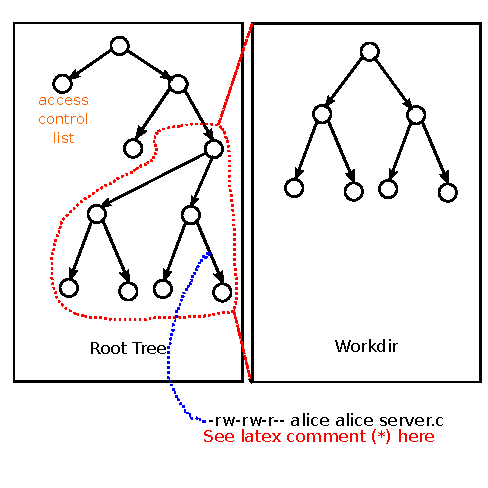
\includegraphics{fig/datamodel.pdf}}
\caption{The relationship between root tree and workdir in \sys.}
\label{f:data-model}
\end{figure}

\endinput

(*) We need a better way to represent the content on the edge. Mike, do you have
any advice?



Figure \ref{f:data-model} shows the structure of the root tree, as well as the
relation between the workdir and the corresponding root tree in the repository.
In \sys, similar to \git data model, a tree is an abstraction of the state
of a directory, and a blob is an abstraction of the state of a regular file. A
tree may have multiple tree entries, which point to subtrees and blobs. Unlike
\git, \sys records access permission information in each tree entry, as depicted
in the figure. \sys also stores some addtional access control information in the
access control list. This paper will discuss about the access control things
in a later section.

In the figure, the user is working on the client side holding the workdir, and
the server, as the storage of the repository, holds the root tree. The user is
only able to view a subset of the root tree. Unlike \git, the user only holds the
current working directory, instead of the whole commit history in the
repository. The next subsection will discuss how \sys performs version control
actions in this model.
\HP{Mike, is the "B checks whether B holds all commits" still a problem? I
think B does not need to check that in this model.}

\subsection{Server Client Model}

It is much easier to solve the access control problem for version control in a
server client model than in a fully distributed model.\HP{Talk about this in
the discussion session or an appendix. See notes/distributed-model.txt for some
discussions.} \hw{Summarize brief reasons here.}

Basically, a server serves as the role of an administrator. The server side
program of \sys (a.k.a \Sys Daemon) has the permission to access any files in a
repository stored on the server. The client side program, on the other hand, can
only access the files that the user has permissions to access. \HP{Remind the
readers to see the next subsection for more details.} The access control is
guaranteed by \sys, which will be described in the next subsection.

When the user wants to access a subset of files via \sys client, the client
sends a request to the \Sys Daemon, and the \Sys Daemon will perform a related
action. If the client needs to checkout a subset of files, \Sys Daemon will
perform a partial checkout action; if the client needs to commit a subset of
files, \Sys Daemon will perform a partial commit action. The details of the
actions \Sys Daemon could perform is in Section \ref{s:daemon}.

\subsection{Access Control Model}
\label{ss:access-model}

The motivation scenarios suggest that \sys should have an access control method
throughout both the time and the space. \hw{Check with section 2.}
Therefore, \sys uses a two dimensional \HP{Any good word here?} way to record
access control information. One dimension is the access permissions in each
file, the other dimension is an access control list in each commit.

The access info\HP{Is this phrase good?} in each file is \unix-like.
Figure 3-a \hw{TODO draw the graph} shows a sample of the access permission
information of several files in a directory. Figure 3-b\hw{TODO draw the graph}
shows how the access
permission information is stored in the backend \git database.

The access info is the typical mechanism for access control in systems
without version control. However, as motivation case \textred{XXX} suggests\HP{
shall we put an example here?}, access control should be not only
throughout\HP{good word?} the space, but also throughout the time. Since the
commit history represents the time span in a version control system, \sys
records an access control list in each commit, which controls access permissions
throughout the time.

\begin{figure}[htb]
%\goodcitationsize
\small
\rule{\linewidth}{.08em}

global: alice bob catherine david \\
development: alice bob david \\
graphics: alice catherine \\

% MW: replacing with more common spelling

\rule{\linewidth}{.08em}
\caption{A sample of access control list}
\label{f:access-list}
\end{figure}

\endinput



Figure \ref{f:access-list} shows the content of an access control
list sample. The access control list contains the "group status" at the commit
point. The group status contains the list of users that belong to the group.

In each checkout or commit action, \Sys Daemon calls the access control part to
checkout whether a file is allowed to be accessed by the user. Figure
\textred{XXX} shows the pseudo code of it.\HP{Do we need pseudo code here?}
For each file, \sys retrieves the access info of the file, and the access
control list info from the commit. It checks the permission in the following
ways:

(1) If the user is the owner of the file, check if the file's "user read" or
"user write" bit is set.

(2) If the user is not the owner of the file, and it belongs to the group of the
file in the access control list, check if the file's "group read" or "group
write" bit is set.

(3) If the previous two conditions are not met, check if the file's "global
read" or "global write" bit is set.

The process then returns whether the user has the permission to access the file,
correspondingly.

\hw{TODO Describe how it solves motivation case \#1}

\subsection{Branch Mode Model}

Branch mode provides a similar functionality to two basic VCS functionalities:

(1) Branch mode can perform a checkout on an old commit in the history.

(2) As the name tells, branch mode can be used to create a branch.

However, branch mode in \sys also has several differences from regular VCSs.
\hw{Describe differences, or remove the sentence.}

The command format for entering branch mode is \textit{backtrace-start relative\_path
branch commit\_id}. The command does the following two things.

(1) Performs a partial checkout for relative\_path and commit\_id.

(2) In the future, when FVM needs to make a commit, it makes a partial
commit for relative\_path to branch, and makes a partial commit for files
not in relative\_path to "master" branch. Figure \ref{f:branch-mode} shows how
it works.

The command format for exiting branch mode is \textit{backtrace-stop branch
option}. The option indicates the destiny of the branch. If the option is
"abandon", the branch will hide into the history without affecting the
mainstream\HP{or "master" branch}. If the option is "overwrite", the most recent
commit (a.k.a head) in the mainstream will be replaced by the head of the
branch. If the option is "merge", \sys will try to merge the head of the branch
with the head of the mainstream, and the user may need to deal with the
conflicts manually, just as \git does.

An interesting point here is that a conflict only happens when multiple users
are working on the same directory. In other words, no conflicts will happen if a
user is the only one working in the repository. In fact, the option "merge" and
"overwrite" has the same effect in single user mode. The reason is that when a
file in a workdir is marked as in branch mode, all further updates of the file
will be commited into the specified branch, which results in that the mainstream
does not have any update of the file during the branch mode period. As a result,
during the merge process, \sys will only take the most recent update of those
files, which are in the specified branch.

\hw{The following several paragraphs needs some work.}
The reason we combine the two things together is that we do not want the
user to enter a "detached head" mode like in \git\cite{git}.\HP{precise
citation needed.} There are two reasons we do not want to do that: First, it is
difficult to manage a subset of files (or a commit) without giving it a branch
name. Second, since the user does not explicitly operate on each branch (we will
see it in the future), the user will lose track of the files if they do not
belong to any branch.

The most important usage for branch mode is to hide changes. When a user
uses branch mode, the changes of files in relative\_path go to a specified
branch, which is not explicitly visible by other users. Only the user's local
machine explicitly sees those changes, until the user merge the branch to
"master" branch. So branch mode could also be called "local mode".

Another usage for branch mode is to separate files. For example, a user can
let his OS configuration files to be always in branch mode. When the OS
configuration is corrupted due to mal-function, a inconsistent update or virus,
the user can checkout previous commit for the OS configuration files without
affecting all the other files.


\iffalse
We described this in the previous section.
\subsection{Trace Level and Automatic Commit}
\hw{Mention trace level and automatic commit stuff if we have space. This
subsection should be relatively short. This is unimportant.}
\fi

